\defChapterTarget{Aggregazione dei risultati}
Calcolando la media per singola tipologia di euristiche possiamo avere un quadro
più approfondito di quali siano i punti di forza e debolezza del sito.
\section{\textbf{Navigazione}}
L'analisi della Navigazione è composta dalla valutazione di cinque elementi.\\
\textbf{\underline{Media: }}(8.0 + 7.7 + 8.3 + 5.3 + 7.7)/5 = 7.4 \\
La Navigazione presentando la media più alta tra le tre tipologie di euristiche è sicuramente
l'aspetto più riuscito del sito, ma rimane comunque un'ampia possibilità di miglioramento.

\section{\textbf{Contenuti}}
L'analisi dei Contenuti è composta dalla valutazione di due elementi.\\
\textbf{\underline{Media: }} (5.7+6.0)/2 = 5.9\\ L'utente trova sempre risposta alla sue
domande, ma spesso i contenuti proposti dal sito sono sovrabbondanti e
confusionari.


\section{\textbf{Layout}}
L'analisi del layout è composta dalla valutazione di quattro elementi.\\
\textbf{\underline{Media: }}(8.9 + 6.7 + 6 + 7.7)/4 = 7.1\\
Il layout è stato giudicato complessivamente in maniera positiva anche se
esistono diversi elementi da migliorare, come scritto nella conclusione. 
\section{\textbf{Aggregazione complessiva}}
Di seguito è possibile trovare un grafico 
    con le medie dei voti dei valutatori per ogni euristica.
    \begin{figure}[H]
        \centering
        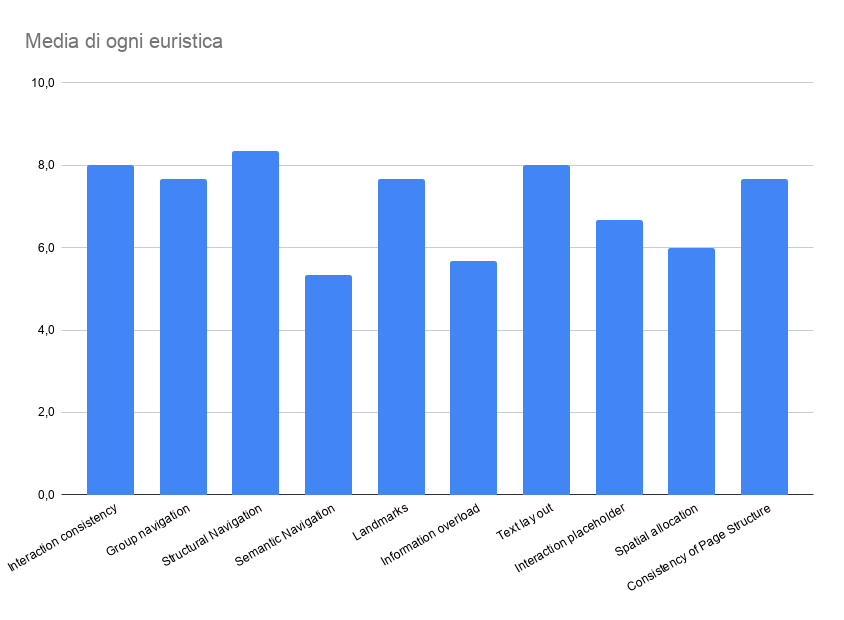
\includegraphics[scale=0.43]{resources/images/graficoMedieEuristiche.png}
    \end{figure}

